\documentclass[12pt,a4paper]{article}
\usepackage[utf8]{inputenc}
\usepackage[spanish]{babel}
\usepackage{amsmath}
\usepackage{amsfonts}
\usepackage{amssymb}
\usepackage{graphicx}
\usepackage[left=2cm,right=2cm,top=2cm,bottom=2cm]{geometry}
\author{Enciso Guerrero Benjamin Salvador\\
Barajas Morales Martin\\
Contreras Juarez Leonardo\\
Negrete Hernandez John\\
Carlos Enrrique Moran Garabito\\
Cinematica De Robots }
\title{Segundo avance.}
\begin{document}
\maketitle

\includegraphics[scale=1.8]{upzmgg.jpg} 
\newpage
\textbf{Introduccion.}
\\\\
Un robot puede ser definido como una máquina que efectúa un número de trabajos, mediante la programación previa. Una peculiaridad de los robots es su estructura de un brazo mecánico y otra su adaptabilidad a diferentes herramientas.
\\\\
Por siglos el ser humano ha construido máquinas que imiten las partes del cuerpo humano. Los antiguos egipcios unieron brazos mecánicos a las estatuas de sus dioses. Estos brazos fueron operados por sacerdotes, quienes clamaban que el movimiento de estos era inspiración de sus dioses. Los griegos construyeron estatuas que operaban con sistemas hidráulicas, los cuales se utilizaban para fascinar a los adoradores de los templos.
\\\\
El uso de sistemas robóticos en la industria, para cumplir funciones que requieren extrema precisión ha ido en ascenso en las últimas décadas como también en el uso personal y familiar.
\\\\
El desarrollo de estos sistemas se ha enfocado en mejorar ciertos aspectos como resistencia para trabajar en diferentes condiciones, precisión con la que se realizan movimientos, multifuncionalidad (manipulación, corte, perforación, etc.), adaptabilidad en diferentes entornos de trabajo.
\\\\
Por lo tanto, dados todas estas utilidades, el diseño propio y construcción de prototipos de brazo robótico para manipulación, corte láser o escaneo tengan un costo accesible tanto para la industria como para la educación, es un buen tema a considerar como proyectos de desarrollo, por estudiantes de ingeniería mecatrónica.
\\\\
El desarrollo en la tecnología, donde se incluyen las computadoras, los actuadores de control retroalimentados, transmisión de potencia a través de engranes, y la tecnología en sensores han contribuido a flexibilizar los mecanismos autómatas para desempeñar tareas dentro de la industria. La investigación en inteligencia artificial desarrolló maneras de emular el procesamiento de información humana con computadoras electrónicas.
\newpage
\title{JUSTIFICACION.}
\\\\
El hecho de soldar de manera automatizada con microalambre va a resolver problemáticas importantes para el dueño, tales como la reducción de tiempo muerto entre soldar dos materiales y ensamblar piezas o esmerilarlos para quitar la escoria y dejar la soldadura limpia, esto podrá ser un proceso semiautomático o automático que sea menos dependiente de la habilidad de operador.
\\\\
Un factor importante en el proyecto es usar MIC/MAC ya que es intrínsecamente más productiva que la soldadura MMA en la que se hace una parada cada vez que se consume el electrodo además de hacer poca formación de gases contaminantes y tóxicos.
\\\\
Las principales bondades de este proceso son la alta productividad y excelente calidad; en otras palabras, se puede depositar grandes cantidades de metal (tres veces más que con el proceso de electrodo revestido) con una buena calidad.
\\\\\\\\
META.
\\\\
Incorporar una soldadora de micro alambre en un brazo robótico
\\\\
\\\\
OBJETIVOS.
\\\\
1-•	Reducción del tiempo al soldar.
\\
2-•	Soldadura más pulcra.
\\
3-•	Ambiente más limpio para el trabajador.
\newpage
\title{Angulos.}
\\\\
Para el brazo se presenta una articulación con movimiento rotacional y dos angulares. Aunque el brazo articulado puede realizar el movimiento llamado interpolación lineal (para lo cual requiere mover
simultáneamente dos o tres de sus articulaciones), el movimiento natural es el de interpolación por articulación, tanto rotacional como angular.
\\\\
Se denomina cinemática directa a una técnica que es utilizada en gráficos 3D por computadora, para solucionar y calcular la posicion de partes de una estructura articulada a partir de sus elementos fijos y las transformaciones que se provocan por las articulaciones de la estructura.
\\\\
La cinemática inversa se refiere a la utilización de las ecuaciones cinemáticas de un robot
para determinar los parámetros comunes que proporcionan una posicion deseada del efector
final. 
\\\\
Especificación del movimiento de un robot de manera que su extremo efector logra una
tarea deseada es conocido como planificación de movimientos. La cinemática inversa transforma el plan de movimiento en trayectorias del actuador en conjuntos para el robot.\\\\

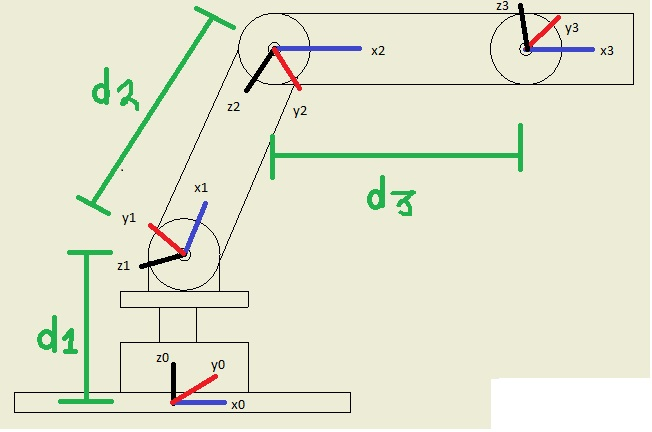
\includegraphics[scale=1]{angulos.jpeg} 
\\
Figura 1.0 Diagrama de flujo con respecto a los angulos.
\\\\
Se realizó el boceto 2D el cual se realizó para sacar los ángulos y la distancia del robot como se muestra en la figura 1.0.
\\\\
Robot antropomórfico con 3 grados de libertad.
el robot se moverá en X y Y, así realizando los movimientos que se les indiquen ya que este se le colocara las pinzas de la soladura por encima del robot.
\\\\
-El apartado de los (i) es el número de los eslabones que tiene el robot.
\\
-La (di) es la distancia que tiene cada ángulo entre sí.
\\
-El (0, a) es la rotación de los codos y articulaciones.
\\\\\\
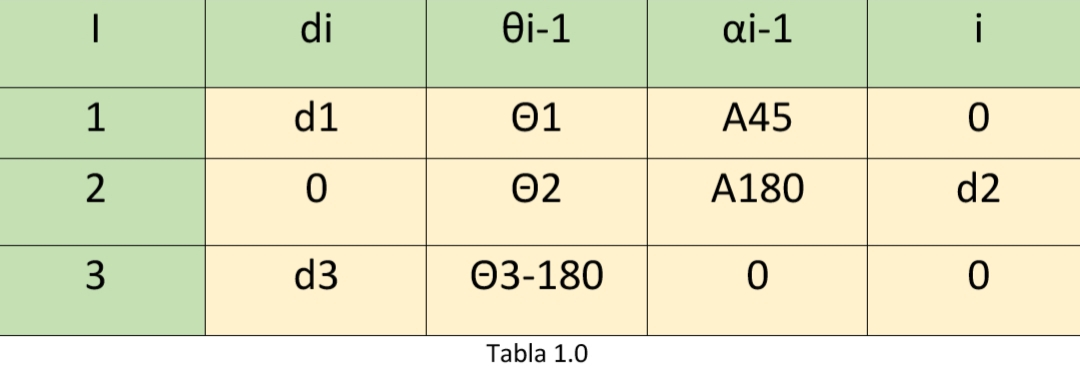
\includegraphics[scale=0.4]{tabla1.jpeg} 
\\\\\\\\
Inventor.
\\\\\\
Para la creacion de la piezas utilizamos el programa Inventor 20 descargado de la paguina oficial.
\\\\
Se realizaron algunas figuras iniciando con la base (Figura 1.0).
\\\\
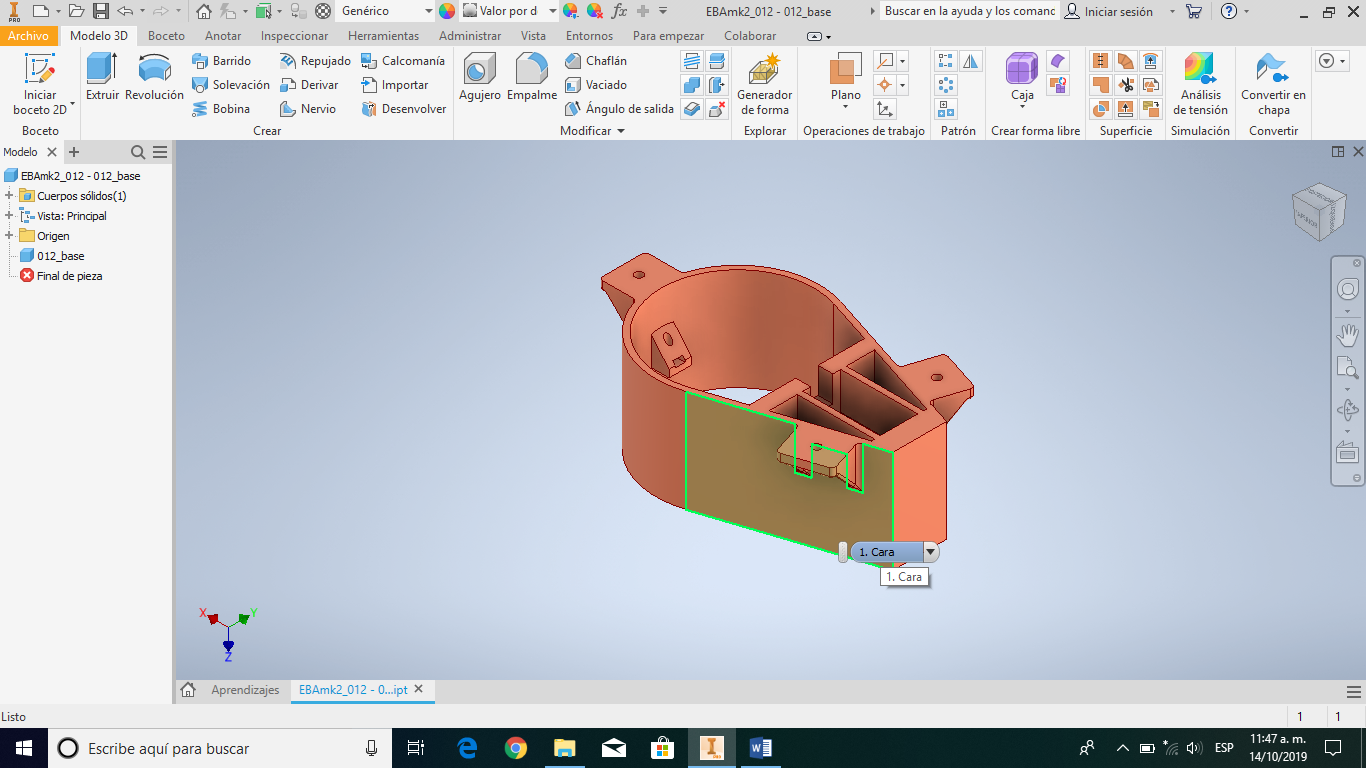
\includegraphics[scale=0.5]{base 1.png} 
\\
Figura 1.1 Base del motor.
\newpage

Hubo complejidades al hacer el diseño ya que teníamos que simular el motor. 
\\\\
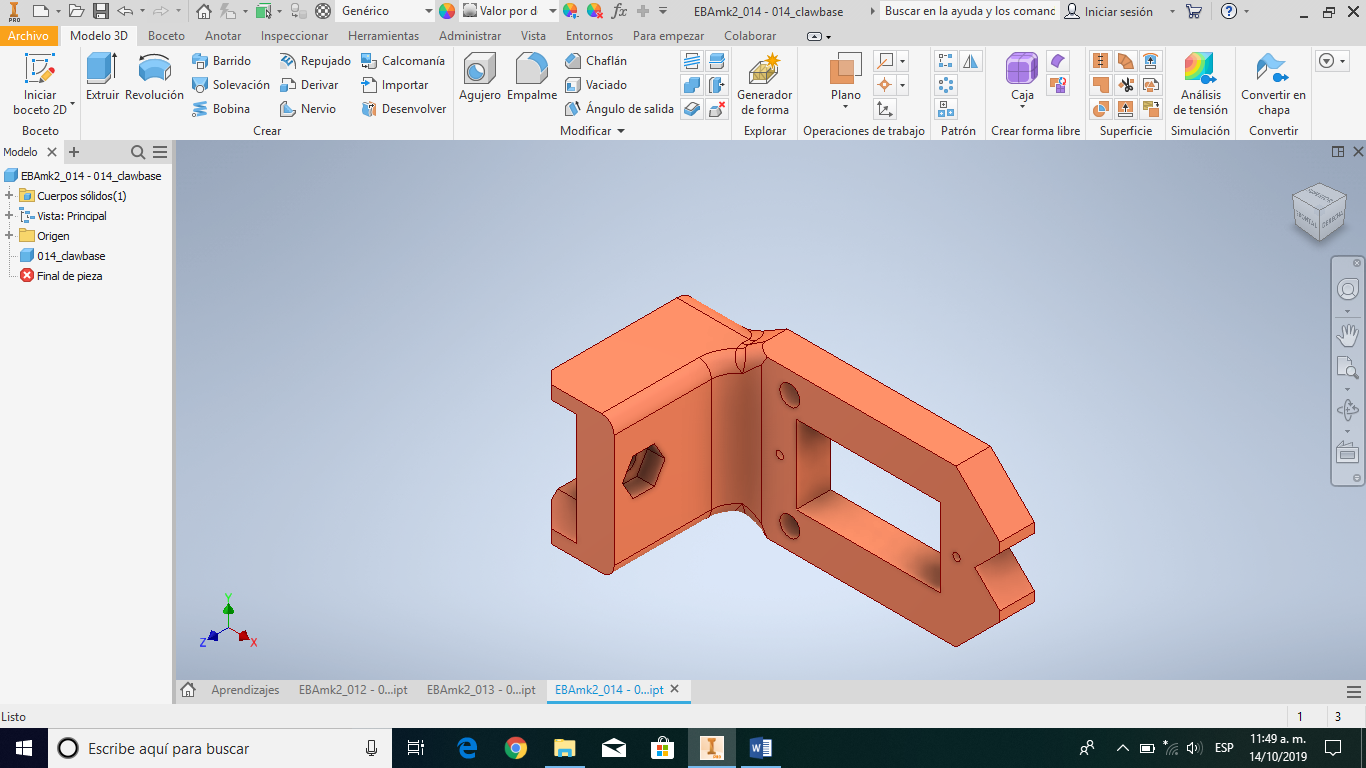
\includegraphics[scale=0.5]{base2.png} 
\\
Figura 1.2 soporte para motor.
\\\\\\\\
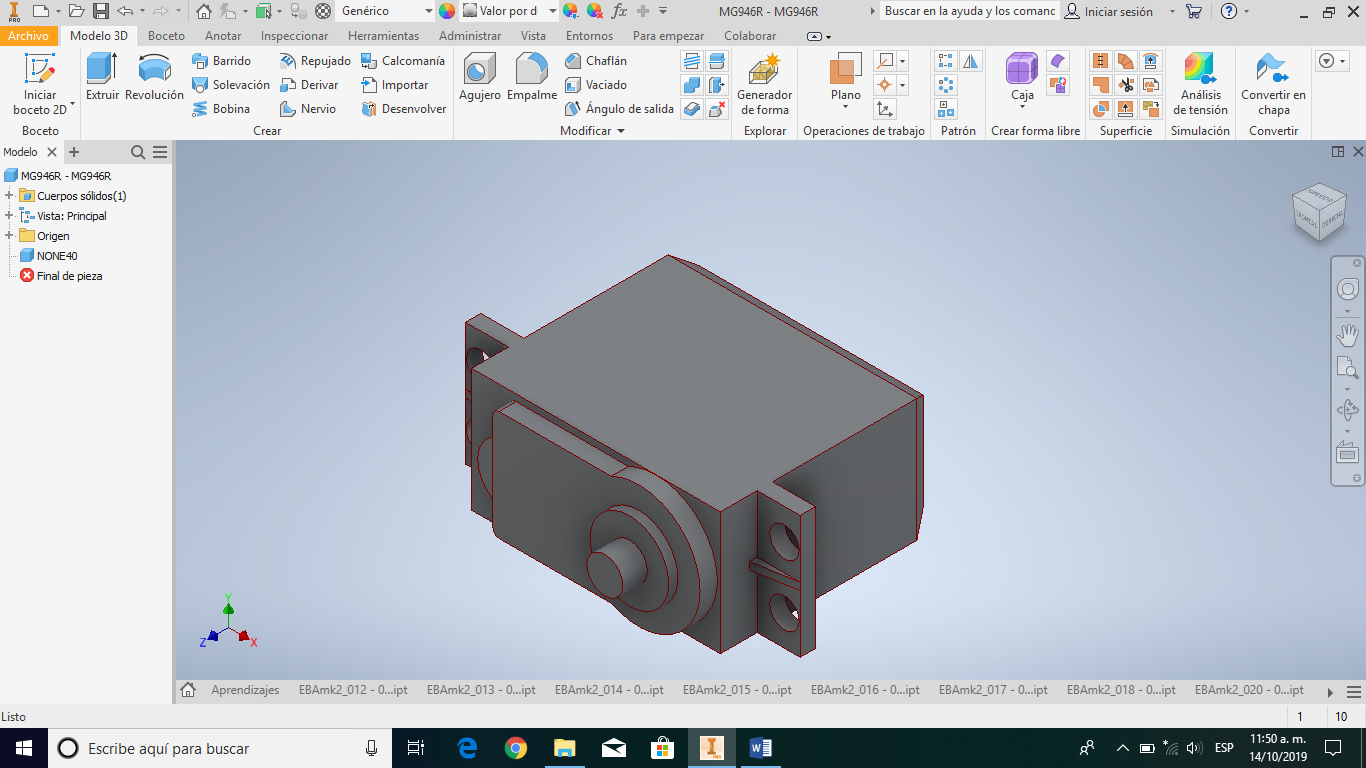
\includegraphics[scale=0.5]{base3.png} 
\\
Figura 1.3 motor.

\newpage
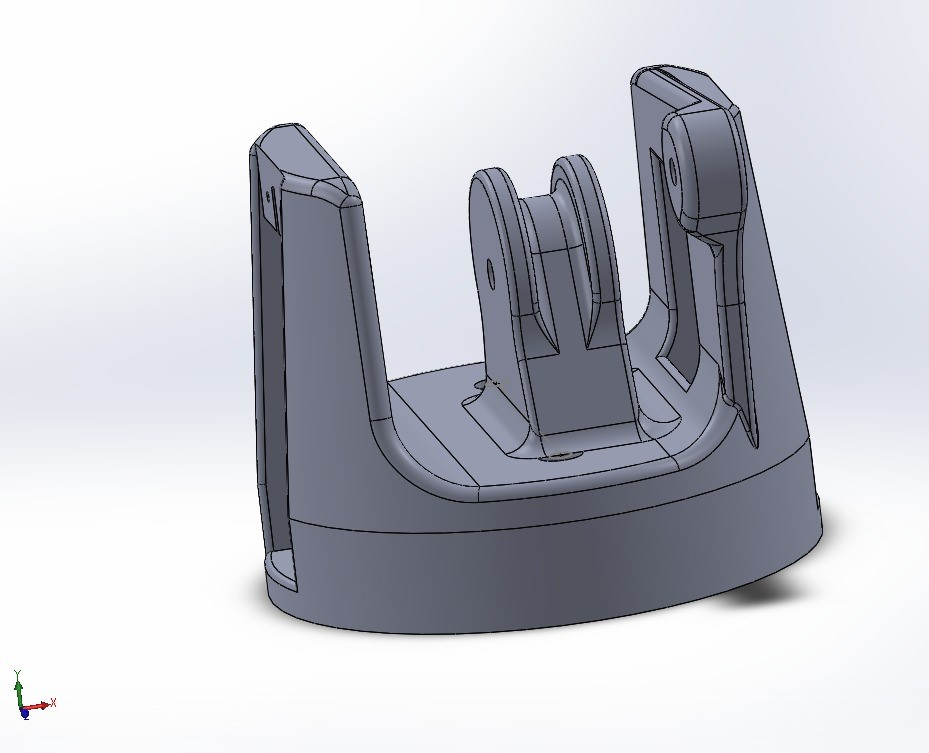
\includegraphics[scale=0.7]{base4.jpg} 
\\
Figura 1.4 base del primer eslabón.


\end{document}